\chapter{Introducción} \chapterlabel{Informe/1-Introduccion} \label{cap:Introducción}

La levitación magnética es un fenómeno físico en el que se aprovecha la fuerza generada por un campo magnético sobre un objeto imantable para mantenerlo en suspensión estática sin contacto mecánico, contrarrestando la acción de la gravedad. Los sistemas que emplean este principio son de gran interés debido a que permiten reemplazar algunos sistemas mecánicos reduciendo significativamente las pérdidas de energía y desgaste de componentes ocasionados por el roce, además de ser más suaves y menos ruidosos.

Sin embargo, no es posible conseguir un estado de levitación magnética al enfrentar, sobre el eje vertical, a un imán permanente y a un objeto ferromagnético situado por debajo. Si bien se puede producir un instante de equilibrio en el que la fuerza magnética de atracción generada por el imán cancele la del peso del objeto haciéndolo levitar, cualquier mínima perturbación haría que ambos se peguen o se separen.

Entre los distintos sistemas que se utilizan para lograr una levitación magnética se encuentra el llamado Electromagnetic Suspension (EMS), en los que se reemplaza el imán permanente por un electroimán. Estos dispositivos tienen la capacidad de generar una fuerza magnética de módulo variable según la intensidad de corriente que circule por él. Como se verá en el desarrollo del proyecto, el fenómeno de levitación presenta una alta inestabilidad, por lo tanto es necesario utilizar un sistema de control que actúe apropiadamente sobre la corriente, regulando la fuerza de atracción y manteniendo el objeto en una suspensión estable. En este documento se aborda el diseño de cada una de las etapas que componen a este sistema de control junto con el diseño de su circuito impreso. 

Una de las aplicaciones más importantes y conocidas que tienen los sistemas EMS es en trenes que utilizan este fenómeno para guiarse e impulsarse, conocidos como ``MagLev''. Los vagones levitan sobre la vía mediante una fuerza magnética de atracción generada por electroimanes colocados en su parte inferior, como se  observa en la figura \ref{fig:img_tren}. 


\begin{figure}[H]
	\centering
	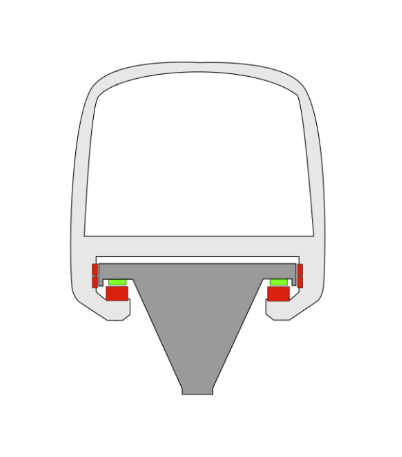
\includegraphics[scale = 0.85]{tren.png}
	\caption{Aplicación de levitación magnética.}
	\label{fig:img_tren}
\end{figure}

\section{Contexto del proyecto}

El desarrollo del sistema de levitación magnética planteado para este proyecto surge como idea de la cátedra Sistemas de Control de la carrera de Ingeniería Electrónica. Su objetivo es disponer de una planta de control con la  que se puedan realizar prácticas en clase. Una primera versión de este dispositivo fue diseñada y construida por la cátedra. Los desarrolladores de este proyecto tuvieron la oportunidad de realizar pruebas y modificaciones durante el cursado de la asignatura. Sin embargo, no se pudo lograr que funcionara correctamente al finalizar la cursada. Por este motivo, se propuso hacer una revisión y rediseño de todas las etapas que componen al sistema en el marco de un proyecto final.

Para la asignatura Sistemas de Control resulta de interés el estudio y experimentación con un sistema de levitación magnética ya que integra varios conceptos dictados durante la cursada y otros aprendidos en el transcurso de la carrera. 

El proyecto comenzó a desarrollarse en junio del 2020. Inicialmente tenía como objetivo el diseño y la construcción de un prototipo funcional que permitiera a los alumnos de la asignatura de Sistemas de Control realizar mediciones y observar el comportamiento de las distintas etapas que componen el sistema. Sin embargo, debido a los retrasos ocasionados por la pandemia (COVID-19), los costos asociados a la fabricación de la placa de control y sus componentes, sumado a la  necesidad de no extender indefinidamente el proyecto, se optó por acotar el alcance sólo al modelado teórico de todas las etapas y al diseño del circuito impreso.

Se espera que en el futuro se pueda construir el sistema de levitación magnética para que sirva como herramienta para los alumnos, de forma tal que les permita experimentar y afianzar los conceptos teóricos adquiridos durante el transcurso de la cursada.


\section{Descripción del dispositivo}
El sistema de control de levitación magnética que se desarrolla en este proyecto tiene la finalidad de mantener en estado de levitación a un objeto por medio de la utilización de un electroimán y una placa de control. El primero consta de dos piezas formadas por láminas de acero apiladas: una con forma de “E” , que se encuentra fijada desde arriba y tiene un bobinado de cobre en su rama central. Esta es la encargada de generar la fuerza magnética. La otra pieza tiene forma de “I”, la cual se mueve libremente sobre el eje vertical y es atraída por la primera mediante su campo magnético. De esta forma, para hacer levitar el objeto se lo sujeta de esta última pieza, como se muestra en la figura \ref{fig:img_Esquema-del-producto}. La distancia de separación entre ambas piezas del electroimán se denomina  \textsl{gap} de aire ($Y_{g}$).

\begin{figure}[H]
	\centering
	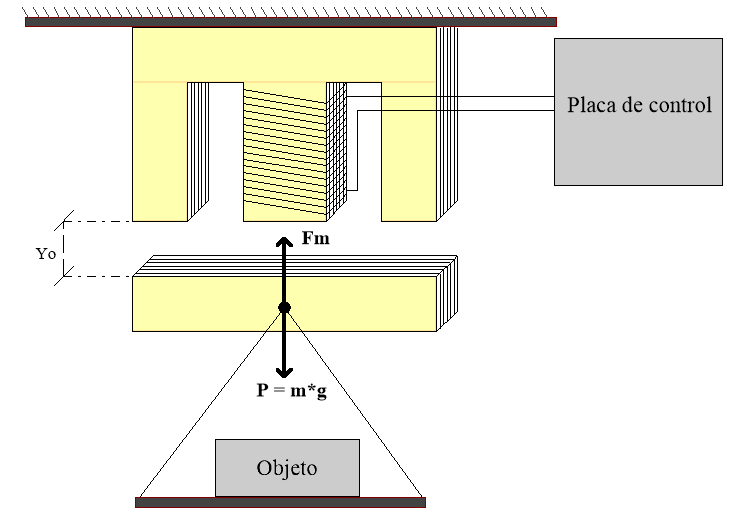
\includegraphics[width=\textwidth]{esquema-del-producto.png}
	\caption{Esquema del dispositivo.}
	\label{fig:img_Esquema-del-producto}
\end{figure}

La circulación de corriente por la bobina genera líneas de campo magnético que recorren la pieza “E” y se cierran a través del aire, de manera similar a un imán permanente. De esta forma, al colocar la pieza “I” en cercanías de este campo se genera una fuerza de atracción entre ambas, cuyo módulo depende de la intensidad de corriente en el bobinado y de la distancia que las separa.

Al hacer circular una corriente constante por el bobinado del electroimán se genera una fuerza proporcional a ella. Es posible encontrar un valor de corriente determinado en el que la fuerza magnética sea igual en módulo a la del peso del objeto, pero con sentido contrario. En este caso, es posible mantener al objeto en estado de levitación. Sin embargo, ante mínimas perturbaciones en la distancia de separación o en la intensidad de la corriente, haría que la fuerza cambie en módulo y que la cancelación de fuerzas deje de ser exacta, provocando que ambos se peguen o que la pieza con forma de “I”, junto con el objeto, se caigan. 

Como se desea mantener fija la distancia de separación entre las piezas que componen al electroimán, es necesario poder compensar las perturbaciones mencionadas anteriormente.   Esto se logra midiendo y realimentando dicha distancia de manera de poder ajustar la fuerza magnética ejercida. Para ello, se actúa sobre la intensidad de la corriente que circula por su bobinado de forma tal que, si el objeto se aleja, la corriente aumentará para acercarlo y evitar que este caiga. De lo contrario, si el objeto se acerca, la corriente disminuirá, para evitar que se pegue al electroimán. 

Es importante destacar que el dispositivo solo puede ejercer control de la posición sobre el eje vertical, por lo que las desviaciones de posición en el eje horizontal no pueden ser controladas y pueden provocar un comportamiento no deseado.

El sistema de control está conformado por las etapas que se muestran en la figura \ref{fig:img_diagrama-en-bloques-del-sistema}. Integra dos controladores distintos: uno analógico y otro digital. Cada uno de ellos se compone de un compensador y un estimador de posición. El usuario decide cual de estas implementaciones ejerce el control mediante la utilización de un \textsl{switch}, por lo que solo una estará activa al mismo tiempo. El sistema digital está implementado en un microcontrolador.

\begin{figure}[H]
	\centering
	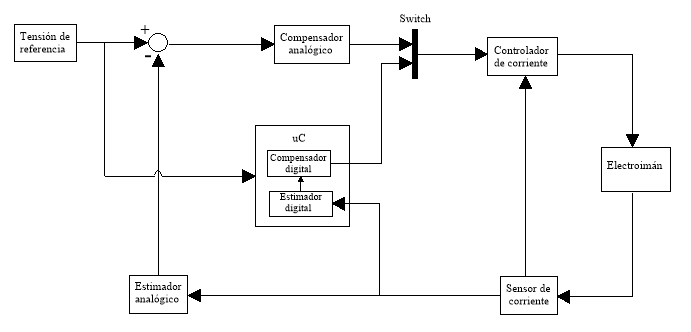
\includegraphics[width=\textwidth]{diagrama-en-bloques-del-sistema.png}
	\caption{Diagrama en bloques del sistema.}
	\label{fig:img_diagrama-en-bloques-del-sistema}
\end{figure}

El estimador de posición se encarga de entregar una tensión proporcional al \textsl{gap} de aire real a partir de la corriente que circula por el electroimán. El usuario puede modificar el \textsl{gap} según desee al variar la tensión entregada por un potenciómetro presente en la placa de control. Tanto la implementación analógica como la digital reciben esta entrada que es comparada con la estimación y luego, su resultado, es utilizado como entrada para el compensador.

Debido a que la planta es naturalmente inestable, como se analizará en el capítulo \ref{cap:CaracterizacionElectroiman}, se utiliza un compensador para lograr la estabilidad y la distancia de separación deseada. En su entrada recibe la comparación de la referencia de posición con la estimación y en base a ella modifica la corriente que ingresa al electroimán, y por ende la fuerza que este ejerce.

El controlador de corriente cumple la función de adaptar los niveles de tensión de salida del compensador a niveles de corriente aptos para que el electroimán genere la fuerza suficiente para sostener el objeto que se hace levitar.


\section{Alcance del proyecto}

El objetivo de este proyecto es realizar un diseño teórico de un sistema de levitación magnética a partir de un electroimán de laminación normalizada con núcleo tipo “E''. La pieza con forma de ”I”, que sujeta al objeto, debe mantenerse en estado de levitación mediante el control de la fuerza magnética generada por la pieza en forma de “E”.

Los requerimientos del proyecto son:

\begin{itemize}
\item Permitir que la distancia de separación $Y_{g}$ entre ambas piezas del electroimán sea ajustable entre $3\:mm$ y $5\:mm$.
\item Mantener en estado de levitación objetos con peso entre $1\:kg$ y $30\:kg$ para todo el rango de distancias de separación.
\item Regular la fuerza electromagnética mediante un sistema de control analógico y otro digital. Solo una de estas implementaciones debe estar  activa al mismo tiempo y el usuario debe poder decidir cuál de ellas ejercerá el control.  Cada sistema debe incluir una etapa de compensación y otra de estimación de la distancia de separación.
\item Realizar la implementación digital mediante un microcontrolador.
\item Diseñar el circuito impreso del sistema de control.
\end{itemize}


\section{Organización del informe}

El informe está dividido en 8 capítulos. En ellos se aborda el diseño teórico y circuital de cada una de las etapas mostradas en la figura \ref{fig:img_diagrama-en-bloques-del-sistema} junto con sus respectivas simulaciones.

En este capítulo se hizo una breve introducción al fenómeno de levitación magnética, y se describió el dispositivo que se diseñará en este trabajo, con sus respectivas especificaciones. En el capítulo 2 se detallan las características constructivas que posee el electroimán y se realiza un modelado físico del fenómeno de levitación para obtener expresiones útiles para el posterior diseño de cada etapa y determinar el comportamiento dinámico del sistema. En el capítulo 3 se diseña y modela el circuito encargado de controlar la corriente que circula por el electroimán. En el capítulo 4 se detalla la estrategia utilizada para realizar la estimación de posición a partir de la corriente del electroimán. En el capítulo 5 se analiza la dinámica de la planta y se utilizan distintas estrategias para conseguir que el sistema presente el comportamiento deseado. En este capítulo 6 se realiza el diseño de un compensador y estimador en el dominio digital para ser implementados en un microcontrolador. En el capítulo 7 se mencionan los criterios tenidos en cuenta para el diseño del circuito impreso y se muestran los esquemáticos e imágenes del PCB desarrollado. Finalmente, en el capítulo 8, se mencionan las conclusiones y aprendizajes obtenidos en el transcurso del proyecto.

 